\section{Octree\-Auxiliary.h File Reference}
\label{OctreeAuxiliary_8h}\index{OctreeAuxiliary.h@{OctreeAuxiliary.h}}
{\tt \#include \char`\"{}Array.h\char`\"{}}\par
{\tt \#include \char`\"{}Vector3r.h\char`\"{}}\par


Include dependency graph for Octree\-Auxiliary.h:\begin{figure}[H]
\begin{center}
\leavevmode
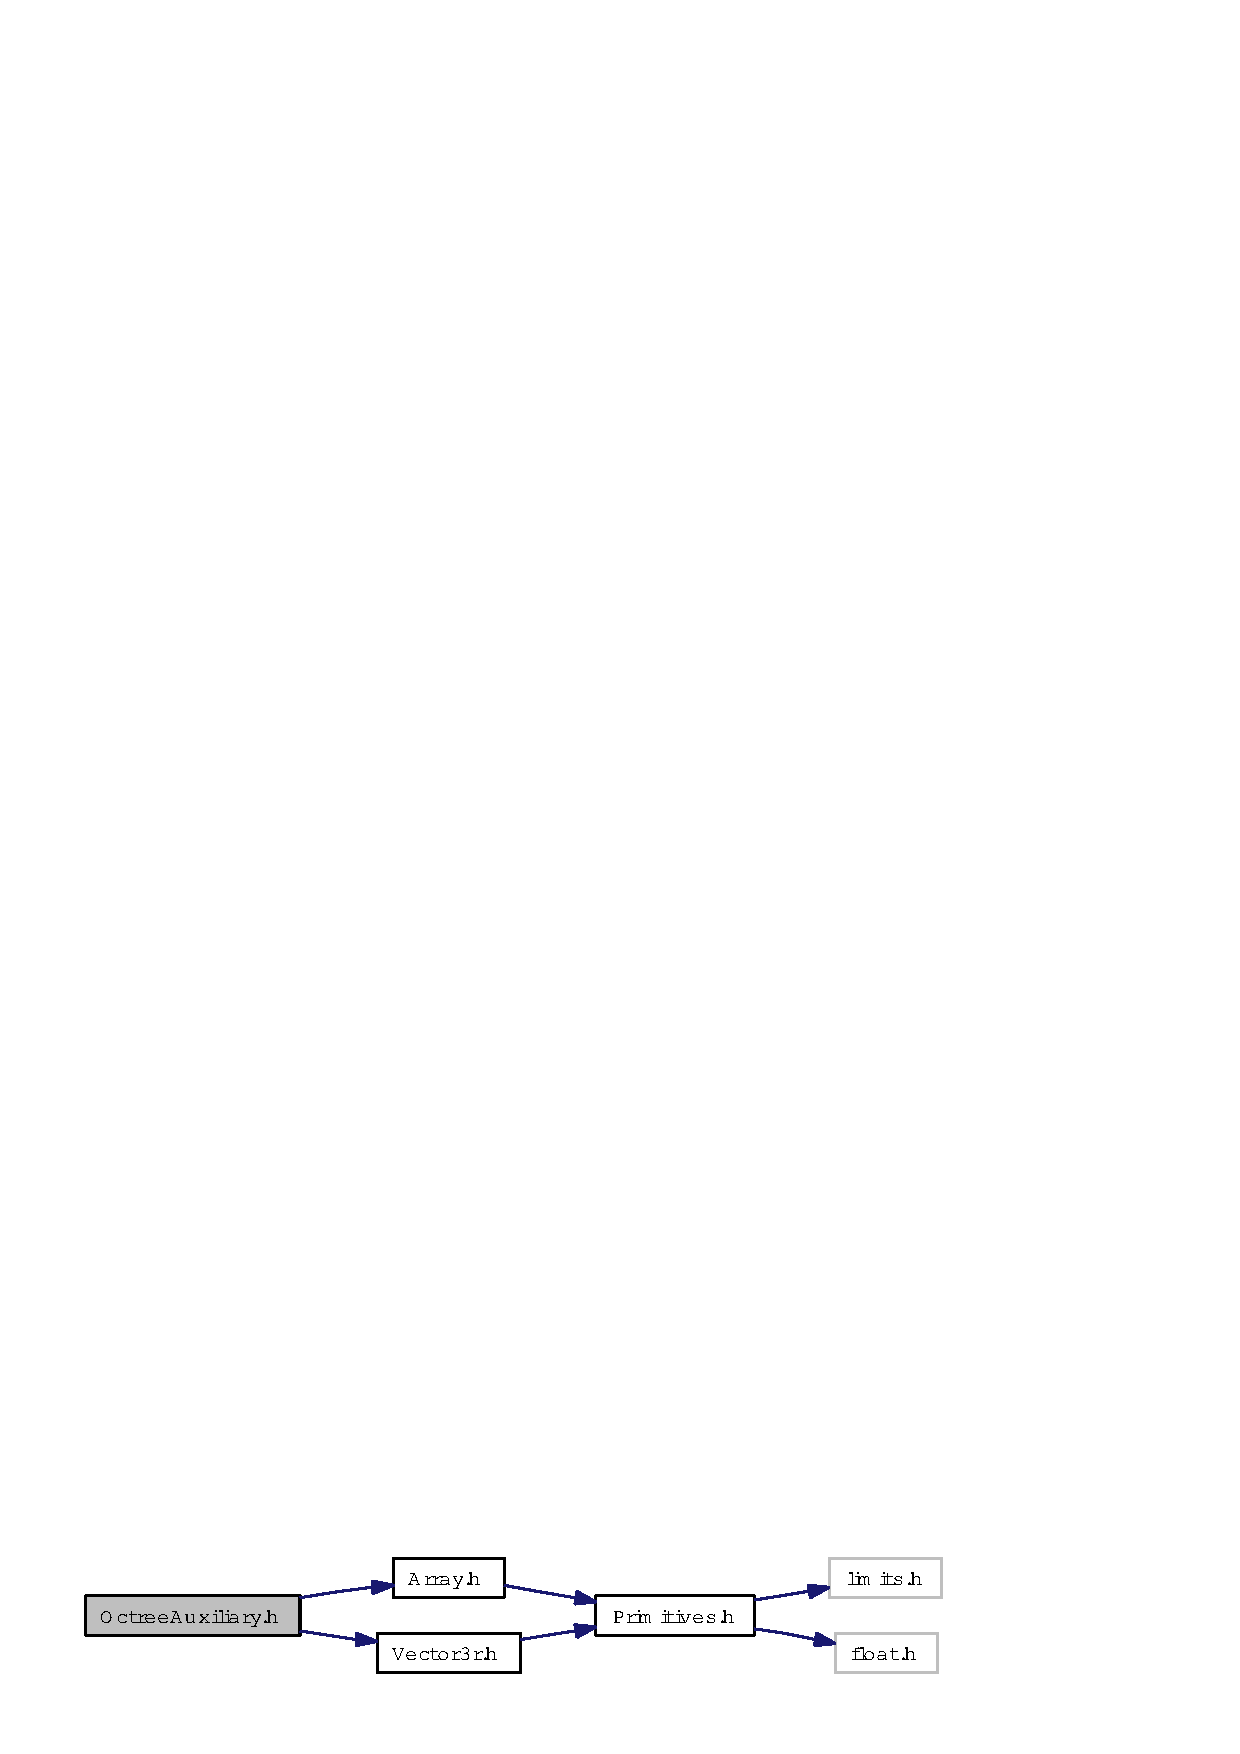
\includegraphics[width=228pt]{OctreeAuxiliary_8h__incl}
\end{center}
\end{figure}


This graph shows which files directly or indirectly include this file:\begin{figure}[H]
\begin{center}
\leavevmode
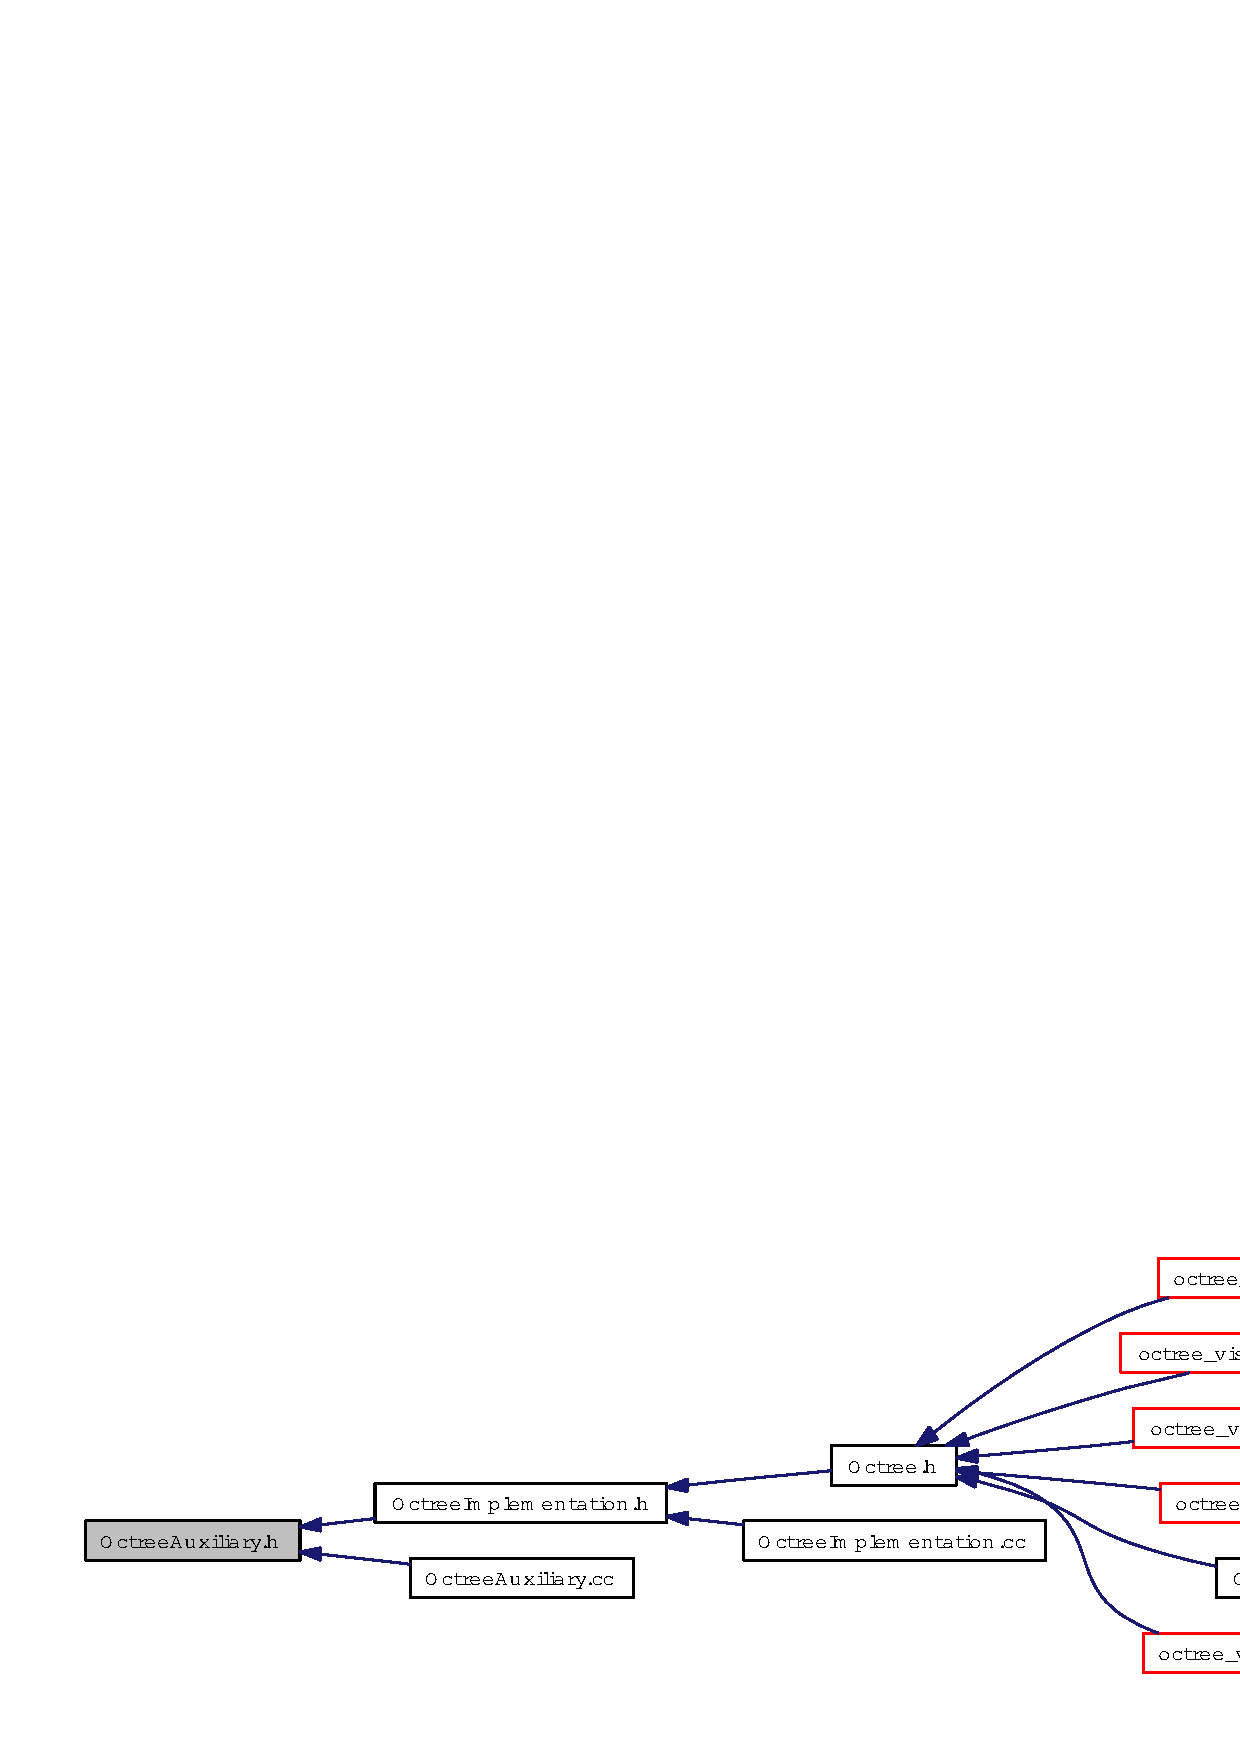
\includegraphics[width=349pt]{OctreeAuxiliary_8h__dep__incl}
\end{center}
\end{figure}
\subsection*{Namespaces}
\begin{CompactItemize}
\item 
namespace {\bf hxa7241\_\-graphics}
\end{CompactItemize}
\subsection*{Classes}
\begin{CompactItemize}
\item 
class {\bf hxa7241\_\-graphics::Octree\-Dimensions}
\item 
class {\bf hxa7241\_\-graphics::Octree\-Bound}
\item 
class {\bf hxa7241\_\-graphics::Octree\-Data}
\item 
class {\bf hxa7241\_\-graphics::Octree\-Agent\-V}
\item 
class {\bf hxa7241\_\-graphics::Octree\-Visitor\-V}
\end{CompactItemize}
